\documentclass[11pt,a4paper]{book}

\usepackage{Appunti}

\begin{document}
\title{Clean Code\\
\large{\textit{Robert C. Martin}}}
\author{Jacopo De Angelis}
\maketitle

\pagebreak
\tableofcontents
\pagebreak

\chapter{Clean code}
Il codice non finirà con l'era dell'autogenerazione da IA. Qualcuno dovrà creare le IA, qualcuno dovrà imparare come dare le specifiche. Il codice sarà sempre presente.

\section{Pessimo codice}
Una delle prime cause del pessimo codice è la fretta dettata dall'ansia. L'idea di dover far uscire il codice il prima possibile ci porta a commettere errori, commettere inesattezze. Quello è ciò che può portare a seri problemi successivamente, il rileggere il proprio codice scritto in maniere quantomeno esecrabili è una tortura. E ricordiamo che se si pensa "lo metto a posto dopo", dopo equivale a mai.

I rallentamenti derivanti da nuovo codice di bassa qualità sono esponenziali, lentamente la produttività crolla perchè operare sul codice precedente è sempre più complicato.
\begin{figure}[h!]
	\begin{center}
		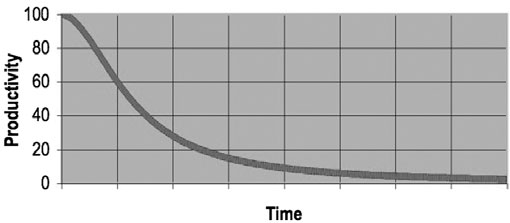
\includegraphics[scale=0.6]{img/001.png}
		\caption{Produttività vs tempo}
		\label{fig: 001}
	\end{center}
\end{figure}

Il che può portare ad un desiderio di ricreare da zero l'intera base del codice, cosa non solo dispendiosa ma che richiede anche molto tempo. I team si trovano a lavorare in parallelo, il nuovo team che ricrea tutto e integra il nuovo lavoro del vecchio team e, alla fine, ci si troverà nella stessa situazione.

\section{Scrivere buon codice}
Scrivere buon codice richiede disciplina nell'uso di molte piccole tecniche applicate in ogni singolo momento. Tutto questo richiede anche una parte di "senso estetico", un percepire il perchè un bel codice sia, appunto, bello.

Una regola che possiamo ereditare dai boy scout: lascia il campo più pulito di come l'hai trovato. Ad esempio: una variabile può avere un nome più autoesplicativo? Cambiala. Una funzione può essere spezzata in più funzioni elementari? Dividila.

\chapter{Nomi significativi}
\section{Usare nomi che rivelino l'intenzione}
Trovare nomi significativi non è semplice ma il tempo che prendono nel farlo è sicuramente meno di quello speso a decifrare nomi non chiari.

Ogni nome, che sia di variabile o di funzione, deve rispondere alle domande:
\begin{itemize}
	\item[] Cosa fa
	\item[] Perchè esiste
	\item[] Come viene utilizzata
\end{itemize}
Se un nome richiede un commento allora il nome è sbagliato.

Ad esempio
\lstinputlisting[language=]{code/001}\label{code: 001}
d non dice molto come nome. Dovremmo scegliere un nome migliore, ad esempio
\lstinputlisting[language=]{code/002}\label{code: 002}
Scegliere un nome che rivela un intento rende molto più semplice cambiare e comprendere un codice. Ad esempio cosa fa questo pezzo di codice?
\lstinputlisting[language=]{code/003}\label{code: 003}
Il problema di questo codice non è la sua semplicità ma la sua capacità di avere un senso implicito. Ad esempio, le domande che ci possiamo porre sono:
\begin{itemize}
	\item[] Cos'è theList?
	\item[] Che significato ha l'elemento 0 di theList?
	\item[] Qual è il significato di 4?
	\item[] Come viene usata la lista ritornata?
\end{itemize}

Queste risposte dovrebbero essere nel codice. Immaginiamo ora di lavorare a campo minato. Rinominiamo la lista con gameBoard.

Ogni cella della board è rappresentata da un array, il valore alla posizione 0 è la posizione dello status della cella e se è 4 vuol dire "segnata". Già dando implicitamente queste notazioni possiamo migliorare il codice:
\lstinputlisting[language=]{code/004}\label{code: 004}

Possiamo andare anche oltre e scrivere una semplice classe per le celle invece di avere degli int. Può includere una funzione con un nome che ne sveli l'intento per nascondere questo numero. Il risultato è:
\lstinputlisting[language=]{code/005}\label{code: 005}

\section{Evitare la disinformazione}
Mai usare parole che non descrivono la realtà, ad esempio usare accountList solo se effettivamente ci troviamo davanti ad una List.

Non usare nomi che variano tra di loro per dei piccoli dettagli, ad esempio \emph{XYZControllerForEfficient\textbf{Handling}OfStrings} e \emph{XYZControllerForEfficient\textbf{Storage}OfStrings}

Avere una naming convention consistente è essenziale. Un pessimo esempio di uso è quello di o ed l minuscoli, pericolosamente simili a 0 e 1.

\section{Fare distinzioni significative}
Evitare nomi con degli errori di battitura intenzionali perchè si vogliono nominare due variabili allo stesso modo. Evitare anche nomi che non danno informazioni, ad esempio:
\lstinputlisting[language=]{code/006}\label{code: 006}

Evitare nomi "che creano rumore", ad esempio ProductInfo e ProductData si differenziano per la seconda parola ma comunque non sappiamo cosa facciano.

Il tipo di entità non dovrebbe mai essere contenuto nel nome. NameString non ha senso, non ci chiederemmo mai se un semplice Name possa essere un float, questo perchè il nome stesso ci informa del suo contenuto.

Un esempio di confusione è:
\lstinputlisting[language=]{code/007}\label{code: 007}
Come potremmo mai sapere quale funzione chiamare dal suo nome?

Distinguere sempre i nomi in modo da intuire immediatamente la loro funzione leggendoli.

\section{Usare nomi pronunciabili}
Devi poterlo pronunciare. Hai mai provato a discutere della funzione della classe Genymdhms (generation date, year, month, day, hour, minute, and second)? Spero di no.

Immaginiamo comparare questa classe
\lstinputlisting[language=]{code/008}\label{code: 008}
con questa
\lstinputlisting[language=]{code/009}\label{code: 009}

\section{Usare nomi ricercabili}
Le variabili con nome di una singola lettera vanno bene solo come variabili locali di un metodo, mai in altro modo, sarebbe impossibile cercarle altrimenti.

Compariamo
\lstinputlisting[language=]{code/010}\label{code: 010}
con
\lstinputlisting[language=]{code/011}\label{code: 011}

\section{Prefissi}
I prefissi erano utili anni fa, ormai sono abbastanza inutili.

\section{Interfacce e implementazione}
Ci sono due scuole di pensiero:
\begin{enumerate}
	\item Interfaccia che inizia con I, implementazione senza decorazioni (IClasse, Classe)
	\item Interfaccia senza decorazioni, implementazione con suffisso Imp (Classe, ClasseImp)
\end{enumerate}

É uguale.

\section{Evitare il mapping mentale}
Il significato dei nomi non deve essere chiaro solo a chi scrive ma anche a chi legge.

\section{Nomi delle classi}
Le classi dovrebbero essere nomi o frasi di sostantivi, evitare Manager, Processor, Data o Info. Una classe non dovrebbe essere un verbo

\section{Nomi dei metodi}
I nomi dovrebbero contenere un verbo che descrivere cosa fanno, ad esempio postPayment, deletePage o save.

Accessori, mutatori e predicati dovrebbero iniziare con get, set e is.

\section{Non usare nomignoli}
Non chiamare variabili, metodi e classi con nomi che utilizzano inside joke, riferimenti culturali o battute. Chiamare la funzione delete() holyHandGranade non è simpatico, è un inferno.

\section{Una parola per concetto}
Scegli una parola che esprima un concetto e mantienila. Ad esempio scegli tra fetch, retrieve e get e poi usa solo quella, non alternare tra le tre.

\section{Usare nomi del dominio di soluzione}


\end{document}